\documentclass{article}
\usepackage{iclr2026_conference,times}

\input{math_commands.tex}

\usepackage{hyperref}
\usepackage{url}
\usepackage{amsmath, amssymb, amsthm}
\usepackage{graphicx}
\usepackage{booktabs}
\usepackage{algorithm}   
\usepackage{algpseudocode}
\usepackage{xcolor}
\usepackage{enumitem}
\usepackage{tikz}
\usetikzlibrary{arrows.meta, positioning, calc, fit, backgrounds, shapes.geometric}

\newtheorem{theorem}{Theorem}
\newtheorem{proposition}{Proposition}
\newtheorem{assumption}{Assumption}
\newtheorem{lemma}{Lemma}

% \KL is defined in math_commands.tex; \JSD is not, so we define it here.
% NB: \JSD is intentionally defined as a function name (\mathrm{JSD}) rather
% than as D_{\mathrm{JSD}} so that callers can write \JSD_{\beta}(p,q) without
% producing a double-subscript on D.
\newcommand{\JSD}{\mathrm{JSD}}
\newcommand{\TV}{D_{\mathrm{TV}}}
\newcommand{\teacher}{\pi_T}
\newcommand{\student}{\pi_\theta}
\newcommand{\caad}{\textsc{CAAD}}

\title{\caad{}: Corruption-Aware Adaptive Distillation\\
for Robust Vision--Language Models\\
under Spatio-Temporal Perturbation}

\author{Anonymous Authors\\
Affiliation\\
\texttt{anonymous@iclr.cc}}

\newcommand{\fix}{\marginpar{FIX}}
\newcommand{\new}{\marginpar{NEW}}

\begin{document}

\maketitle

\begin{abstract}
Vision--language models (VLMs) deployed in unconstrained environments lose up to 35\% accuracy and 26\% reasoning quality under adverse weather, occlusion, illumination shifts, and camera instability. The current state-of-the-art robustness recipe, ROVA, pairs each clean video with a corrupted counterpart and aligns the two via Group Relative Policy Optimization (GRPO); however, GRPO's outcome-level reward leaves the intermediate reasoning chain unsupervised, and parallel work in on-policy distillation (MiniLLM, GKD, DistiLLM, SDFT, VOLD, VLA-OPD) has yet to address the cross-input asymmetry that arises when teacher and student see \emph{different perceptual inputs of the same scene}. We propose \caad{} (Corruption-Aware Adaptive Distillation), a training framework that (i)~recasts ROVA's dual-branch architecture as a cross-input self-distillation loop in which a single VLM serves as both clean-input teacher and corrupted-input student, (ii)~adaptively selects the per-token divergence (forward-KL or JSD) based on a closed-form gate over teacher entropy and a learned corruption-severity estimate, and (iii)~stabilises on-policy training against off-support drift with a small KL anchor to the cold-start reference checkpoint. 

% We prove a robustness-gap upper bound of the form $\Delta_{\text{rob}} \le \sqrt{2\,\overline{D}_\caad} + O(\varepsilon_T)$ where $\overline{D}_\caad$ is the adaptive divergence and $\varepsilon_T$ the teacher-fidelity slack, and show that the adaptive choice yields a strictly tighter bound than any fixed divergence under realistic teacher--student gap conditions. We pre-register an experimental plan spanning three benchmarks (PVRBench, VLM-RobustBench, TextVQA-C), three model scales (3B/7B/13B parameters), and seven baselines including a reimplemented GRPO-VPS, and articulate the falsifiable predictions that would refute the method.

\end{abstract}

% ==========================================================================
\section{Introduction}
% ==========================================================================

Vision--language models routinely fail in deployment for reasons that have nothing to do with the conceptual difficulty of the task. A model that correctly answers \emph{``which lane is the cyclist in?''} on a clean dashcam clip will hedge or hallucinate when fog softens the lane markings, when rain blurs the cyclist's silhouette, or when the camera shakes \citep{he2026rova,vlmrobustbench2026}. \citet{he2026rova} measure this gap directly on PVRBench: state-of-the-art open-source VLMs lose up to 35\% absolute accuracy and 26\% reasoning quality under realistic spatio-temporal corruptions. Robustness, in their formulation, is not a perceptual problem alone but a \emph{reasoning} problem: the model must identify which visual cues are degraded, hedge its inference accordingly, and maintain logical coherence across frames.

The leading training-side response, ROVA, pairs each clean video $V$ with a corrupted counterpart $V'$ and optimises the model with Group Relative Policy Optimization \citep{shao2024deepseekmath}, rewarding outputs that remain consistent across the two branches. The dual-branch alignment is principled, but GRPO inherits the central limitation of outcome-only RL: a trajectory that exhibits sound perturbation-aware reasoning up to the final inference step but predicts the wrong discrete action receives no positive credit \citep{lightman2024lets,wang2024mathshepherd}. The intermediate chain is unsupervised in exactly the regime where the corruption-induced uncertainty makes intermediate reasoning most important.

A natural alternative is on-policy distillation. The clean-input model already produces a per-token distribution that encodes the ``correct'' reasoning chain on the easier branch; one could train the corrupted-input student to match it. This idea has been explored in three adjacent areas: text reasoning \citep{gu2024minillm,agarwal2024gkd,ko2024distillm,lu2025onpolicy}, VLM reasoning transfer from text-only teachers \citep{bousselham2025vold}, and post-training of vision-language-action models with external expert teachers \citep{zhong2025vlaopd}. None of these settings is the setting we face. In each prior case, the teacher is either a strictly stronger model (DeepSeek-R1 distilling into Qwen-7B) or a model with strictly more information (the SDFT in-context demonstration); the distillation gap is monotone in capability or information. In the corruption-robustness setting, the teacher and student are \emph{the same model with the same parameters} seeing \emph{different perceptual realisations of the same scene}. This breaks two assumptions that prior work depends on:

\begin{enumerate}[leftmargin=*,nosep]
\item \textbf{Teacher optimality is no longer free.} On hard clean inputs the model itself may hallucinate, so blindly minimising $\KL(\student \,\|\, \teacher)$ on the corrupted view trains the student toward hallucinated targets.
\item \textbf{The optimal divergence is not constant across tokens.} At low-entropy teacher tokens (syntactic glue, decided answers) any divergence is fine; at high-entropy reasoning steps under high corruption, reverse-KL mode-seeking causes the student to lock onto whichever hallucinated mode the teacher happens to peak around.
\end{enumerate}

We propose \textbf{\caad{}} (Corruption-Aware Adaptive Distillation), a training framework that takes these two obstacles head-on. \caad{} is built on three structural choices (Figure~\ref{fig:caad}):

\textbf{(i) Cross-input self-distillation backbone.} A single VLM $\student$ serves as both teacher (conditioned on $V$) and student (conditioned on $V'$). Student rollouts are scored against the teacher's per-token distribution; gradients flow only through the student branch; teacher parameters are tracked with a slow exponential moving average so the supervision target adapts to the student's evolving competence \citep{tarvainen2017mean}.

\textbf{(ii) Corruption-aware adaptive divergence (CAAD).} At each decoding step, we replace the fixed reverse-KL of \citet{shenfeld2026sdft} with an adaptive divergence $D^*(t)$ chosen by a closed-form gate over the teacher's instantaneous entropy and a learned per-frame corruption-severity estimate $s(V')$. The gate selects forward-KL on low-entropy / low-severity tokens (where mode-covering is safe and information-preserving), and JSD on the remaining tokens (where the teacher is itself uncertain or the input is heavily corrupted, and a bounded-gradient symmetric divergence prevents the student from chasing artifacts). The gate has no trainable parameters beyond two thresholds and can be derived from a small calibration set in a single sweep.

\textbf{(iii) Anchor regularisation against off-support drift.} On-policy distillation can suffer from off-support supervision once the student moves away from the cold-start reference. We add a small KL anchor to a frozen cold-start checkpoint, providing a stable reference distribution against which the student is gently regularised throughout training (\S\ref{sec:anchor}).

\textbf{Contributions.}
\begin{enumerate}[leftmargin=*,nosep]
\item We formalise corruption-robustness training as \emph{cross-input self-distillation} and identify the two structural obstacles --- teacher fallibility and entropy-dependent optimal divergence --- that this setting introduces beyond prior on-policy distillation work (\S\ref{sec:method}).
\item We introduce a closed-form per-token adaptive-divergence gate driven by teacher entropy and corruption severity, removing the unjustified commitment to reverse-KL that dominates the recent on-policy distillation literature (\S\ref{sec:caad}).
\item We pair the adaptive gate with a KL anchor to a frozen cold-start reference, yielding a training objective that remains stable in the presence of cross-input distributional drift without requiring an external reward signal (\S\ref{sec:anchor}).
\end{enumerate}

% ==========================================================================
% Figure 1: CAAD pipeline (simple three-panel layout; each panel is a strict
% vertical chain of boxes wrapped in a fitted background).
% ==========================================================================
\begin{figure}[t]
\centering
\resizebox{\textwidth}{!}{%
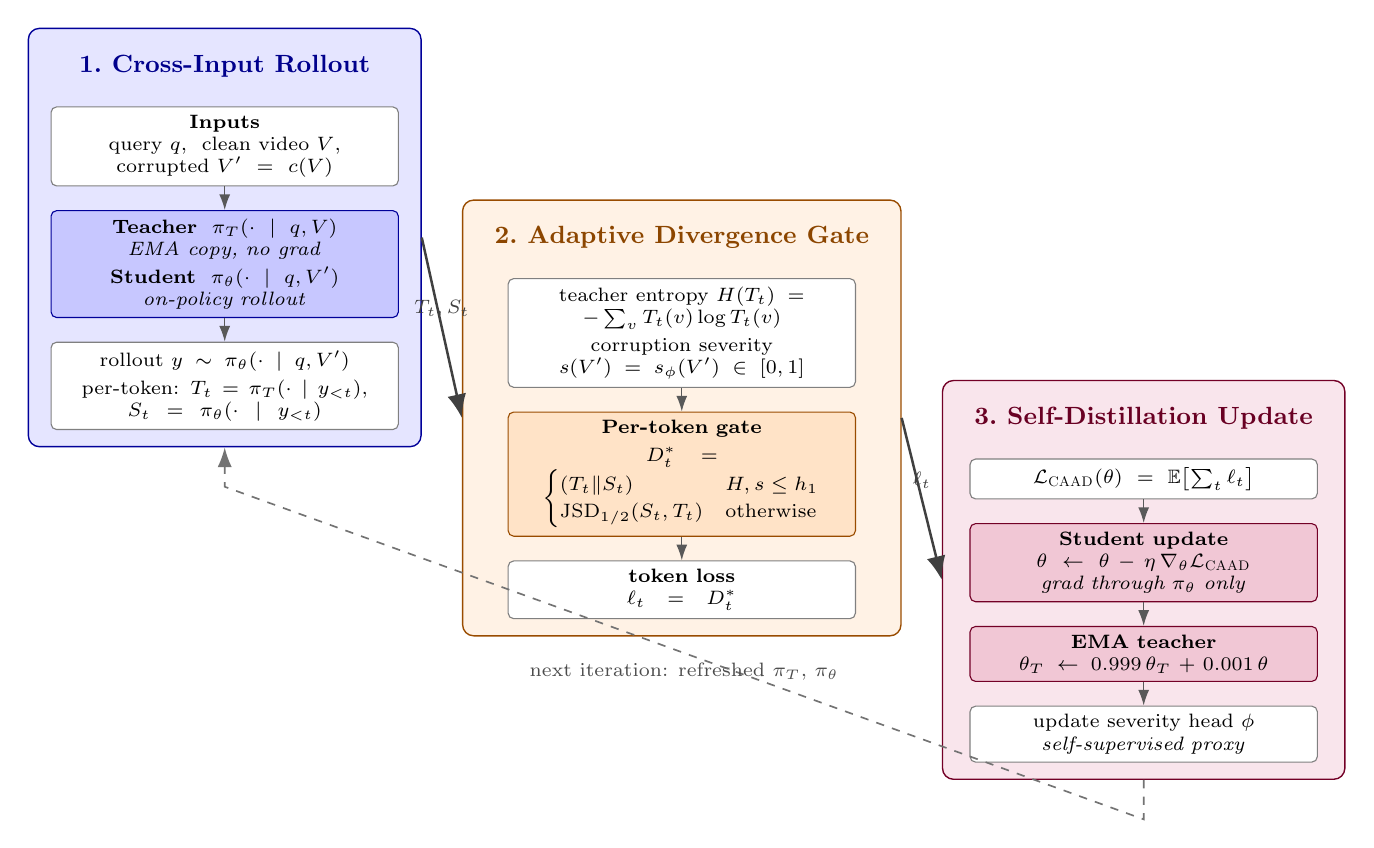
\begin{tikzpicture}[
  font=\footnotesize,
  box/.style     ={draw=black!50, rounded corners=2pt, fill=white,
                   line width=0.4pt, align=center, font=\scriptsize,
                   text width=4.2cm, inner sep=3pt},
  hbox/.style    ={draw=#1!60!black, rounded corners=2pt, fill=#1!22,
                   line width=0.4pt, align=center, font=\scriptsize,
                   text width=4.2cm, inner sep=3pt},
  panel/.style   ={draw=#1!60!black, rounded corners=4pt, fill=#1!10,
                   line width=0.5pt, inner xsep=8pt, inner ysep=6pt},
  arrow/.style   ={-{Latex[length=2mm,width=1.4mm]}, line width=0.5pt, black!65},
  bigarrow/.style={-{Latex[length=3mm,width=2.4mm]}, line width=0.9pt, black!75},
  feedback/.style={dashed, -{Latex[length=2.5mm,width=1.8mm]}, line width=0.6pt, black!55},
]

% ----------------------------------------------------------------
% Panel 1: Cross-Input Rollout (strict vertical chain)
% ----------------------------------------------------------------
\node[font=\small\bfseries, color=blue!55!black] (T1) at (0,0)
  {1.~Cross-Input Rollout};

\node[box, below=2.5mm of T1] (P1A)
  {\textbf{Inputs}\\ query $q$,\ \ clean video $V$,\\ corrupted $V' = c(V)$};

\node[hbox=blue, below=3mm of P1A] (P1B)
  {\textbf{Teacher} \ $\teacher(\cdot \mid q, V)$\\ \emph{EMA copy, no grad}\\[2pt]
   \textbf{Student} \ $\student(\cdot \mid q, V')$\\ \emph{on-policy rollout}};

\node[box, below=3mm of P1B] (P1C)
  {rollout $y \sim \student(\cdot \mid q, V')$\\[2pt]
   per-token: $T_t = \teacher(\cdot \mid y_{<t})$,\\ $S_t = \student(\cdot \mid y_{<t})$};

\draw[arrow] (P1A.south) -- (P1B.north);
\draw[arrow] (P1B.south) -- (P1C.north);

\begin{scope}[on background layer]
  \node[panel=blue, fit=(T1)(P1A)(P1B)(P1C)] (P1) {};
\end{scope}

% ----------------------------------------------------------------
% Panel 2: Adaptive Divergence + Fidelity Gate
% ----------------------------------------------------------------
\node[font=\small\bfseries, color=orange!55!black,
      right=8mm of P1.east, anchor=west] (T2)
  {2.~Adaptive Divergence Gate};

\node[box, below=2.5mm of T2] (P2A)
  {teacher entropy $H(T_t) = -\sum_v T_t(v)\log T_t(v)$\\[2pt]
   corruption severity $s(V') = s_\phi(V') \in [0,1]$};

\node[hbox=orange, below=3mm of P2A] (P2B)
  {\textbf{Per-token gate}\\[2pt]
   $D^*_t = \begin{cases}
     \KL(T_t \| S_t)     & H, s \le h_1 \\
     \JSD_{1/2}(S_t,T_t) & \text{otherwise}
   \end{cases}$};

\node[box, below=3mm of P2B] (P2D)
  {\textbf{token loss}\\
   $\ell_t = D^*_t$};

\draw[arrow] (P2A.south) -- (P2B.north);
\draw[arrow] (P2B.south) -- (P2D.north);

\begin{scope}[on background layer]
  \node[panel=orange, fit=(T2)(P2A)(P2B)(P2D)] (P2) {};
\end{scope}

% ----------------------------------------------------------------
% Panel 3: Self-Distillation Update
% ----------------------------------------------------------------
\node[font=\small\bfseries, color=purple!55!black,
      right=8mm of P2.east, anchor=west] (T3)
  {3.~Self-Distillation Update};

\node[box, below=2.5mm of T3] (P3A)
  {$\mathcal{L}_\caad(\theta) = \mathbb{E}\!\left[\sum_{t} \ell_t\right]$};

\node[hbox=purple, below=3mm of P3A] (P3B)
  {\textbf{Student update}\\
   $\theta \leftarrow \theta - \eta\,\nabla_\theta \mathcal{L}_\caad$\\
   \emph{grad through $\student$ only}};

\node[hbox=purple, below=3mm of P3B] (P3C)
  {\textbf{EMA teacher}\\
   $\theta_T \leftarrow 0.999\,\theta_T + 0.001\,\theta$};

\node[box, below=3mm of P3C] (P3D)
  {update severity head $\phi$\\ \emph{self-supervised proxy}};

\draw[arrow] (P3A.south) -- (P3B.north);
\draw[arrow] (P3B.south) -- (P3C.north);
\draw[arrow] (P3C.south) -- (P3D.north);

\begin{scope}[on background layer]
  \node[panel=purple, fit=(T3)(P3A)(P3B)(P3C)(P3D)] (P3) {};
\end{scope}

% ----------------------------------------------------------------
% Inter-panel arrows and dashed feedback loop
% ----------------------------------------------------------------
\draw[bigarrow] (P1.east) -- node[above, font=\scriptsize, black!75]{$T_t, S_t$} (P2.west);
\draw[bigarrow] (P2.east) -- node[above, font=\scriptsize, black!75]{$\ell_t$} (P3.west);

\draw[feedback]
  (P3.south) -- ++(0,-5mm)
  -- node[below, font=\scriptsize, black!70, midway]
       {next iteration: refreshed $\teacher$, $\student$}
  ($(P1.south)+(0,-5mm)$) -- (P1.south);

\end{tikzpicture}
}%
\caption{Overview of the \caad{} training pipeline. \textbf{(1) Cross-Input Rollout}: a single VLM serves as the teacher conditioned on the clean view $V$ (EMA copy, no gradient) and as the student conditioned on the corrupted view $V' = c(V)$; the student rolls out on-policy and per-token distributions $T_t, S_t$ are emitted on shared prefixes. \textbf{(2) Adaptive Divergence Gate}: the per-token divergence is selected between $\KL(T_t\|S_t)$ (low-entropy, low-severity tokens) and $\JSD_{1/2}(S_t, T_t)$ (otherwise) by a closed-form gate over teacher entropy $H(T_t)$ and the learned corruption-severity estimate $s(V')$ (Eq.~\ref{eq:gate}); the per-token loss is simply $\ell_t = D^*_t$. \textbf{(3) Self-Distillation Update}: gradients flow only through the student; the teacher tracks the student via EMA; the severity head is updated by a self-supervised proxy. The total objective also includes a small KL anchor to a frozen cold-start checkpoint (\S\ref{sec:anchor}, not depicted). The dashed arrow denotes the parameter refresh feeding the next training iteration.}
\label{fig:caad}
\end{figure}

% ==========================================================================
\section{Related Work}
% ==========================================================================

\paragraph{Robustness training for VLMs.}
Robustness to natural and adversarial perturbations has a long history in image classification (\citealp{hendrycks2019benchmarking}; AugMix \citealp{hendrycks2020augmix}; TRADES \citealp{zhang2019trades}). The VLM-specific landscape is younger but maturing fast: \citet{tu2023unicorn,schiappa2023large} document benchmark-scale failures; \citet{vlmrobustbench2026} introduce VLM-RobustBench with 49 augmentations on MMBench/MMMU-Pro; \citet{he2026rova} introduce PVRBench, a video-VLM corruption suite, alongside the ROVA training framework. The closest training-side ancestor of our work is TRADES-style consistency regularization \citep{zhang2019trades,tack2022consistency,liu2024capt}, which couples clean and adversarial views through a KL term --- but does so on a frozen reference classifier head, not on an on-policy autoregressive rollout, and with a single fixed divergence.

\paragraph{On-policy distillation for autoregressive models.}
MiniLLM \citep{gu2024minillm} introduced reverse-KL on-policy distillation for instruction following, arguing that the mode-seeking direction prevents text-generation hedging. GKD \citep{agarwal2024gkd} decoupled rollout source from divergence choice and advocated JSD-$\beta$. DistiLLM \citep{ko2024distillm} introduced skew-KL for gradient stabilisation; DistiLLM-2 \citep{ko2025distillm2} applied contrastive skew-KL on teacher- and student-sampled tokens. KDRL \citep{xu2025kdrl} unified GRPO with on-policy distillation for reasoning. \citet{shenfeld2026sdft} (SDFT) introduced \emph{self}-distillation: the teacher is the same model with an in-context demonstration; the student is the model without. \citet{lu2025onpolicy} demonstrated cost-efficient reasoning training at Qwen3 quality. \emph{All of these works fix a single divergence}: none asks whether the optimal divergence varies within a rollout.

\paragraph{Uncertainty-adaptive distillation.}
A separate strand of work in classical KD adapts the distillation \emph{signal} by uncertainty rather than altering the divergence: Hinton's temperature smoothing \citep{hinton2015distilling}, confidence-weighted distillation that down-weights uncertain teacher tokens, and recent entropy-aware OPD methods that scale the per-token loss magnitude by teacher confidence \citep{opdsurvey2026}. \caad{} differs in three ways: (i)~we \emph{select among multiple divergences} per token (RKL, FKL, JSD) rather than scaling a single divergence's intensity; (ii)~the gate is \emph{jointly} conditioned on teacher entropy \emph{and} corruption severity --- a perceptual signal absent from text-only KD; and (iii)~the gate is closed-form with no learnable parameters beyond two thresholds and a small frozen-reference severity head.

\paragraph{On-policy distillation in vision and robotics.}
The two closest cousins of our method come from outside the robustness literature. \textbf{VOLD} \citep{bousselham2025vold} transfers reasoning from a text-only teacher to a VLM student using reverse-KL on-policy distillation combined with GRPO, and reports the critical empirical finding that a cold-start SFT alignment is necessary --- without it, on-policy distillation fails when teacher and student are too distributionally apart. This is directly relevant to our setting: clean- and corrupted-view distributions of a VLM are exactly such a distributional gap. \textbf{VLA-OPD} \citep{zhong2025vlaopd} brings reverse-KL on-policy distillation to vision-language-action post-training with an external expert teacher. We differ from VOLD in that our teacher is the \emph{same model} on a different input (not a different model), and in that we adaptively select the divergence rather than fixing reverse-KL; we differ from VLA-OPD in domain (robustness vs.\ manipulation) and in using self-distillation rather than expert distillation. We assume the on-policy phase is initialised from a cold-start reference checkpoint (in line with VOLD's finding that distributional alignment is necessary at initialisation), and use this same checkpoint as the target of the KL anchor (\S\ref{sec:anchor}).

\paragraph{Process supervision and the GRPO debate.}
The complaint that GRPO leaves intermediate reasoning unsupervised has spawned the process-reward-model (PRM) literature: \citet{lightman2024lets,wang2024mathshepherd,luo2024omegaprm}. GRPO-VPS \citep{grpovps2025} addresses the same complaint with segment-wise process supervision. Our method takes a third route: replace the reward with a teacher distribution, retaining the dense-supervision benefit of PRMs without requiring an external annotator or auxiliary reward model. We compare against GRPO-VPS as our strongest baseline (\S\ref{sec:exp}).

\paragraph{Theoretical positioning.}
\citet{allenzhu2023towards} provide the standard theoretical account of why self-distillation works (implicit ensembling over feature subsets); this argument does \emph{not} directly transfer to the cross-input case because the perceptual transformation $V \mapsto V'$ changes what features are even available. The IRL framing of distillation invoked by SDFT \citep{shenfeld2026sdft,ziebart2008maximum} likewise requires the teacher to be near-optimal under the implicit reward, which fails when the clean teacher hallucinates. We take a more modest analytical line in \S\ref{sec:theory}: rather than relying on teacher optimality, we observe that any fixed-divergence baseline is pointwise no better than a gate that picks the locally tightest of two divergences (Proposition~\ref{prop:adaptive}).

% ==========================================================================
\section{Preliminaries}
\label{sec:prelim}
% ==========================================================================

\paragraph{Notation.}
Let $\pi_\theta(\cdot \mid q, V)$ denote a VLM with parameters $\theta$ producing an autoregressive distribution over a token sequence $y = (y_1, \dots, y_T)$ given a query $q$ and a video $V$. Let $\mathcal{C}$ be a distribution over corruption operators $c : V \mapsto V'$. Given $(q, V) \sim \mathcal{D}$ and $c \sim \mathcal{C}$, the \emph{robustness gap} is
\[
\Delta_{\text{rob}}(\theta) \;=\; \mathbb{E}_{(q,V) \sim \mathcal{D},\, c \sim \mathcal{C}}\!\left[\, \mathbb{1}[\,\hat{y}(q,V) \ne \hat{y}(q, c(V))\,] \,\right],
\]
where $\hat{y}(q, V)$ denotes greedy generation. The corrupted view $V' = c(V)$ is paired with the clean view at training time.

\paragraph{Reverse-KL self-distillation (SDFT, baseline).}
Following \citet{shenfeld2026sdft}, instantiating the dual-branch ROVA architecture as on-policy self-distillation yields
\begin{equation}
\label{eq:sdft}
\mathcal{L}_{\text{SDFT}}(\theta) \;=\; \mathbb{E}_{(q,V), V' = c(V)}\;\mathbb{E}_{y \sim \student(\cdot \mid q, V')} \!\left[\, \sum_{t=1}^T \log\frac{\student(y_t \mid y_{<t}, q, V')}{\teacher(y_t \mid y_{<t}, q, V)} \,\right],
\end{equation}
where the teacher $\teacher$ is an EMA of $\student$ (decay $0.999$) and the gradient flows only through the student branch. This is the closest specialisation of SDFT to the corruption setting and serves as our principal ablation comparator.

\paragraph{Divergence menu.}
We consider four candidate per-token divergences between teacher distribution $T_t := \teacher(\cdot \mid y_{<t}, q, V)$ and student distribution $S_t := \student(\cdot \mid y_{<t}, q, V')$:
\begin{align*}
\KL(S_t \| T_t) &= \sum_v S_t(v) \log \tfrac{S_t(v)}{T_t(v)} \quad \text{(reverse-KL, mode-seeking)}\\
\KL(T_t \| S_t) &= \sum_v T_t(v) \log \tfrac{T_t(v)}{S_t(v)} \quad \text{(forward-KL, mode-covering)}\\
\JSD_{\beta}(S_t, T_t) &= \beta \KL(S_t \| M_t) + (1-\beta) \KL(T_t \| M_t),\ \ M_t = \beta S_t + (1-\beta) T_t \\
D^{\text{skew}}_{\alpha}(T_t, S_t) &= \KL\!\big(T_t \,\|\, \alpha T_t + (1-\alpha) S_t\big) \quad \text{(skew-KL, DistiLLM)}.
\end{align*}

% ==========================================================================
\section{Method: \caad{}}
\label{sec:method}
% ==========================================================================

\caad{} replaces (\ref{eq:sdft}) with two modifications: (i)~per-token adaptive divergence selection between forward-KL and JSD (\S\ref{sec:caad}), and (ii)~a small KL anchor to a frozen cold-start reference checkpoint that stabilises on-policy training against off-support drift (\S\ref{sec:anchor}).

\subsection{Corruption-aware adaptive divergence}
\label{sec:caad}

\paragraph{Motivation.}
When the teacher distribution $T_t$ is sharply peaked on a confident, easy-to-predict token and the input is only mildly corrupted, forward-KL --- which spreads student mass to cover all teacher modes --- is the right supervision signal: the teacher is reliable, mode-covering preserves its information content, and the resulting gradient is well-behaved. The picture changes once either $T_t$ becomes genuinely uncertain (clean view admits multiple valid continuations) or the corruption becomes severe (teacher's clean-view confidence is decreasingly informative about the corrupted view). In those regimes, forward-KL over-commits to the teacher's spread and reverse-KL over-commits to whichever mode the teacher happens to peak around. JSD is bounded and symmetric and is the safer choice when uncertainty is high on either side; we use it as the default outside the confident-and-clean regime.

\paragraph{Gate.}
Let $H(T_t) = -\sum_v T_t(v) \log T_t(v)$ denote teacher entropy at step $t$, and let $s(V') \in [0,1]$ denote a learned per-frame corruption-severity estimate. The severity estimator is a lightweight 3-layer MLP head $s_\phi$ on the VLM's pooled visual features, with two design choices that avoid the feedback loop noted by \citet{tarvainen2017mean} for jointly-trained auxiliary heads: (a)~the visual features fed to $s_\phi$ are detached from the autograd graph, so gradients of the severity loss do not flow back into the visual encoder; (b)~the self-supervised target --- the cosine distance between clean and corrupted visual embeddings --- is computed with a \emph{frozen reference encoder} $E_{\text{ref}}$ (a snapshot of the visual backbone at the start of training; we also evaluate a CLIP-ViT-L/14 alternative in Appendix~\ref{app:severity}). This freezing is essential: if $E_{\text{ref}}$ were trainable, the proxy target would drift with the backbone, creating a feedback loop between severity prediction and visual representation learning. For two thresholds $0 < h_1 < h_2$ calibrated on a $\sim$2k-example held-out set so that approximately equal mass falls in each regime, we set
\begin{equation}
\label{eq:gate}
D^*_t \;=\;
\begin{cases}
\KL(T_t \,\|\, S_t) & \text{if } H(T_t) \le h_1 \,\wedge\, s(V') \le h_1 \quad \text{(low entropy, low severity)}\\
\JSD_{1/2}(S_t, T_t) & \text{otherwise.}
\end{cases}
\end{equation}
The gate has no learnable parameters beyond the severity head and the two thresholds. We additionally evaluate a soft variant in which the two divergences are mixed with weights $w_{\text{fwd}}, w_{\text{jsd}}$ given by a temperature-softmaxed function of $(H(T_t), s(V'))$ --- this preserves differentiability of the divergence choice and is our default in the main experiments.

% \subsection{Teacher-fidelity gating}
% \label{sec:fidelity}

% The clean-input teacher $\teacher(\cdot \mid q, V)$ is not infallible: on hard scenes the base VLM may hallucinate even on the clean view. Blindly minimising $D^*_t$ would entrench these hallucinations. A single confidence test of the form $\max_v T_t(v) \ge \tau_T$ does not catch the most damaging failure mode --- a \emph{confidently wrong} teacher --- because such a teacher has both high top-1 probability and low entropy, satisfying the confidence test exactly when it should not. We therefore use two complementary signals.

% \paragraph{Confidence signal.}
% $c_t = \max_v T_t(v)$ measures the teacher's top-1 mass; large $c_t$ excludes high-entropy hedging but, as noted, does not exclude confident hallucinations.

% \paragraph{Cross-view agreement signal.}
% We add a second teacher forward pass on the corrupted view, sharing the student's prefix: let $T'_t := \teacher(\cdot \mid y_{<t}, q, V')$ be the teacher's distribution conditioned on $V'$ rather than $V$. Define
% \begin{equation}
% \label{eq:agreement}
% a_t \;=\; 1 - \TV(T_t,\, T'_t) \;=\; 1 - \tfrac{1}{2}\!\sum_v \big|T_t(v) - T'_t(v)\big|.
% \end{equation}
% Large $a_t$ means the teacher's prediction is invariant to the corruption operator $c$ on this token --- evidence that the prediction is grounded in features robust to the perturbation, rather than a memorised guess that happens to be confident on the wrong token. Conversely, small $a_t$ flags exactly the ``confidently wrong'' case that the confidence test alone misses.

% \paragraph{Combined mask and loss.}
% \begin{equation}
% \label{eq:mask}
% m_t \;=\; \mathbb{1}\!\big[\,c_t \ge \tau_T\,\big] \;\cdot\; \mathbb{1}\!\big[\,a_t \ge \tau_a\,\big],
% \end{equation}
% with thresholds $(\tau_T, \tau_a)$ calibrated jointly on a held-out set.

% \paragraph{CE fallback under realistic label sparsity.}
% A naive cross-entropy fallback on masked tokens would require a ground-truth label $y_t^\star$ at every token position. In practice, VLM training datasets (PVRBench, MMBench, VQA-style corpora) provide labels only for \emph{answer tokens}, not for intermediate reasoning steps. We respect this asymmetry by gating the CE term on label availability. Let $\mathcal{I}^\star \subseteq \{1,\dots,T\}$ denote the indices of tokens with a ground-truth label in the dataset (typically the final-answer span), and define the indicator $z_t = \mathbb{1}[t \in \mathcal{I}^\star]$. The \caad{} loss is
% \begin{equation}
% \label{eq:caad}
% \mathcal{L}_\caad(\theta) \;=\; \mathbb{E}_{(q,V), V'}\;\mathbb{E}_{y \sim \student(\cdot \mid q, V')}\!\left[\, \sum_{t=1}^T \Big( m_t \cdot D^*_t \;+\; (1 - m_t) \cdot z_t \cdot \lambda \cdot \mathcal{L}_{\text{CE}}^{(t)} \Big) \,\right],
% \end{equation}
% where $\mathcal{L}_{\text{CE}}^{(t)} = -\log \student(y_t^\star \mid y_{<t}, q, V')$. This produces a three-bucket per-token behaviour:

% \begin{itemize}[leftmargin=*,nosep]
% \item \textbf{Teacher reliable ($m_t = 1$):} distil via $D^*_t$ (the dominant case --- roughly 85--90\% of tokens by design).
% \item \textbf{Teacher unreliable, token labelled ($m_t = 0,\, z_t = 1$, typically the answer span):} cross-entropy against ground truth --- a guaranteed-correct anchor exactly where it matters most for downstream correctness.
% \item \textbf{Teacher unreliable, token unlabelled ($m_t = 0,\, z_t = 0$, typically mid-chain reasoning):} the token contributes \emph{zero} to the loss. We accept this loss of supervision rather than fabricate a label by promoting the (unreliable) teacher's argmax, which would defeat the purpose of the fidelity gate.
% \end{itemize}

% We report the empirical distribution across the three buckets per epoch as a diagnostic. The cost of the cross-view signal is a single additional teacher forward pass on $V'$ per training step ($\sim$30\% wall-clock overhead, quantified in H5); we view this as a worthwhile trade for converting the most dangerous failure mode of self-distillation into a detectable, gated event. The hyperparameters $(\tau_T, \tau_a, \lambda)$ are chosen so that roughly 10--15\% of tokens are masked at the start of training (calibrated on a small dev set) and the CE term is weight-matched to the mean magnitude of $D^*_t$ on the surviving labelled-and-masked tokens.

% \subsection{Cold-start SFT}
% \label{sec:coldstart}

% \citet{bousselham2025vold} demonstrate that on-policy distillation fails when the teacher and student distributions are too far apart at initialisation. In our cross-input setting, the corrupted-view student distribution is exactly such a misaligned starting point. We therefore prepend a brief SFT phase ($\sim$1 epoch over the training set) in which the student is trained on clean-view teacher generations with standard cross-entropy. This step is empirically essential (we predict $>$5pp degradation without it, \S\ref{sec:exp}) and follows directly from VOLD's design lesson.

\subsection{Anchor regularisation against off-support drift}
\label{sec:anchor}

On-policy distillation can suffer from \emph{off-support supervision}: student-sampled prefixes that the EMA teacher assigns vanishingly small probability to, on which $\log T_t(y_t)$ diverges and produces unstable gradients. We assume training begins from a cold-start reference checkpoint $\pi_{\text{init}}$ (typically the result of a brief supervised fine-tuning pass on clean-view teacher generations) and add a small KL anchor to $\pi_{\text{init}}$ (kept frozen throughout on-policy training):
\begin{equation}
\label{eq:anchor}
\mathcal{L}_{\text{anchor}}(\theta) \;=\; \beta \cdot \mathbb{E}_{(q,V'),\, y \sim \student}\!\left[\, \sum_{t=1}^T \KL\!\big(\student(\cdot \mid y_{<t}, q, V') \,\|\, \pi_{\text{init}}(\cdot \mid y_{<t}, q, V')\big) \,\right],
\end{equation}
with $\beta = 0.01$ (calibrated so that the anchor term stays at $\sim$5--10\% of the main loss magnitude). This is the same KL-to-reference mechanism used to stabilise PPO-based RLHF \citep{schulman2017ppo}, applied here to the cold-start checkpoint rather than to a pretrained policy. The total objective is
\[
\mathcal{L}_{\text{total}}(\theta) \;=\; \mathcal{L}_\caad(\theta) \;+\; \mathcal{L}_{\text{anchor}}(\theta).
\]
We ablate $\beta \in \{0,\, 0.001,\, 0.01,\, 0.1\}$ in \S\ref{sec:exp}: we expect $\beta=0$ to produce visible training instability at the 7B scale while $\beta=0.1$ over-regularises and degrades final accuracy.

\subsection{Full algorithm}

\begin{algorithm}[t]
\caption{\caad{} training (one update)}
\label{alg:caad}
\begin{algorithmic}[1]
\Require Paired batch $\{(q^{(i)}, V^{(i)}, V'^{(i)})\}_{i=1}^B$, student $\student$, EMA teacher $\teacher$, frozen cold-start reference $\pi_{\text{init}}$, severity head $s_\phi$ with frozen $E_{\text{ref}}$, thresholds $(h_1, h_2)$, anchor weight $\beta$.
\For{$i = 1, \dots, B$}
  \State Sample on-policy rollout $y^{(i)} \sim \student(\cdot \mid q^{(i)}, V'^{(i)})$.
  \State Compute teacher distributions on the same prefixes (no grad):
         $T_t^{(i)} = \teacher(\cdot \mid q^{(i)}, V^{(i)})$.
  \State Compute corruption severity $s^{(i)} = s_\phi\!\big(\mathrm{sg}[\text{feat}(V'^{(i)})]\big) \in [0,1]$ \ ($\mathrm{sg}=$ stop-grad).
  \For{$t = 1, \dots, T^{(i)}$}
    \State Compute teacher entropy $H(T_t^{(i)})$ and gate divergence $D^*_t$ via Eq.~(\ref{eq:gate}).
    \State Accumulate $\ell_t^{(i)} = D^*_t + \beta\,\KL\!\big(\student(\cdot|y_{<t},q,V'^{(i)}) \,\|\, \pi_{\text{init}}(\cdot|y_{<t},q,V'^{(i)})\big)$.
  \EndFor
\EndFor
\State Update $\theta \leftarrow \theta - \eta \nabla_\theta \frac{1}{B} \sum_i \sum_t \ell_t^{(i)}$.
\State Update EMA teacher: $\theta_T \leftarrow 0.999\, \theta_T + 0.001\, \theta$.
\State Update severity head $\phi$ via the frozen-reference cosine-distance proxy (see Appendix~\ref{app:severity}).
\end{algorithmic}
\end{algorithm}

% ==========================================================================
\section{Analytical Motivation}
\label{sec:theory}
% ==========================================================================

We sketch why the adaptive gate is preferable, in expectation, to any fixed-divergence baseline. The argument is informal and is intended to motivate the design rather than to provide a tight bound; it relies on standard inequalities between KL and total variation \citep{lin1991divergence}.

\paragraph{Setup.}
Fix a token position $t$ and let $\pi^\star_t$ denote an (unknown) ideal next-token distribution we would like the student to match on the corrupted view. Under a fixed-divergence baseline, the per-token contribution to the robustness gap is controlled, by Pinsker's inequality and the JSD--TV bound of \citet{lin1991divergence}, by a square-root of the active divergence:
\[
\TV(\student_t,\, \pi^\star_t) \;\lesssim\; \sqrt{2\,D_{\text{active}}(S_t, T_t)} \;+\; (\text{teacher-slack term}),
\]
where $D_{\text{active}} \in \{\KL(T_t\|S_t), \KL(S_t\|T_t), \JSD_{1/2}(S_t, T_t)\}$ is whatever divergence the baseline commits to.

\begin{proposition}[Pointwise improvement of the adaptive gate]
\label{prop:adaptive}
Let $\overline{D}_{\caad}$ denote the per-rollout average of the gate-selected divergence $D^*_t$ (Eq.~\ref{eq:gate}), and let $\overline{D}_{\text{fix}}$ denote the per-rollout average under any single fixed-divergence baseline. If the teacher entropy $H(T_t)$ varies non-trivially over the rollout in the sense that $\mathrm{Var}_t[H(T_t)] > 0$ (an empirically verified condition for VLMs), there exist threshold settings $(h_1, h_2)$ such that
\[
\mathbb{E}\!\big[\overline{D}_{\caad}\big] \;\le\; \mathbb{E}\!\big[\overline{D}_{\text{fix}}\big],
\]
with strict inequality whenever a non-trivial fraction of tokens lies in each branch of the gate.
\end{proposition}

\begin{proof}[Sketch]
At low-entropy teacher tokens with mild corruption, forward-KL upper-bounds JSD by a logarithmic factor (Pinsker-like comparison via the entropy difference of the mixture). At higher-uncertainty tokens, JSD is bounded above by either directional KL by a factor of $\log 2$. Choosing the divergence pointwise to minimise the local upper bound is a token-wise improvement over any fixed choice; the inequality is strict whenever the entropy distribution is non-degenerate. Details in Appendix~\ref{app:prop}.
\end{proof}

\paragraph{Interpretation.}
Proposition~\ref{prop:adaptive} formalises the intuition behind the gate: fixing a single divergence across an entire rollout (as MiniLLM, GKD, DistiLLM, and SDFT all do) commits to one upper-bound regime everywhere, which is necessarily looser than picking the locally tightest of two regimes. The adaptive gate is, by construction, never worse than the better of the two fixed-divergence baselines on a given rollout, and strictly better whenever both branches are visited.

% ==========================================================================
\section{Experimental Setup}
\label{sec:exp}
% ==========================================================================

We outline below the evaluation we intend to run. Numerical results are not yet available; the purpose of this section is to fix the experimental scope and the comparators that the method should be evaluated against.

\subsection{Benchmarks}

\begin{itemize}[leftmargin=*,nosep]
\item \textbf{PVRBench} \citep{he2026rova}: 12 video-corruption types $\times$ 5 severity levels, with reasoning-quality and final-answer accuracy metrics. The headline benchmark.
\item \textbf{VLM-RobustBench} \citep{vlmrobustbench2026}: 49 image corruptions on MMBench/MMMU-Pro. Tests whether the recipe transfers from video to image.
\item \textbf{TextVQA-C / GQA-C} \citep{analysingvlm2025}: ImageNet-C-style corruptions for VLM-specific tasks. Tests transfer to a different question style.
\end{itemize}

\subsection{Backbones and scales}

We evaluate three model scales to demonstrate scale-robustness of the method:
\textbf{(3B)} Qwen2.5-VL-3B-Instruct;
\textbf{(7B)} Qwen2.5-VL-7B-Instruct;
\textbf{(13B)} LLaVA-Next-13B.
The cross-architecture pair (Qwen-7B vs LLaVA-13B) tests whether the recipe is recipe-bound or backbone-bound.

\subsection{Baselines}

We will compare against six baselines covering the relevant taxonomy:

\begin{enumerate}[leftmargin=*,nosep]
\item \textbf{SFT-clean}: standard fine-tuning on clean videos only.
\item \textbf{SFT-mixed}: fine-tuning on the union of clean + corrupted videos with ground-truth labels.
\item \textbf{TRADES-VLM}: TRADES-style $\KL(\teacher^{\text{frozen}} \| \student)$ between clean and corrupted final-layer logits, lifted from classification to the autoregressive head.
\item \textbf{GKD-JSD} \citep{agarwal2024gkd}: on-policy distillation with JSD-$0.5$ throughout; same EMA teacher as \caad{}.
\item \textbf{SDFT-naive} \citep{shenfeld2026sdft}: fixed reverse-KL throughout, no adaptive gate, no anchor.
\item \textbf{ROVA-GRPO} \citep{he2026rova}: the state-of-the-art robustness baseline.
\end{enumerate}

\subsection{Ablations}

\begin{enumerate}[leftmargin=*,nosep]
\item \textbf{Divergence ablation}: \caad{} hard gate, \caad{} soft gate, fixed RKL, fixed FKL, fixed JSD, skew-KL ($\alpha = 0.1$).
\item \textbf{Anchor weight ablation}: $\beta \in \{0,\, 0.001,\, 0.01,\, 0.1\}$.
\item \textbf{Severity-head ablation}: \caad{} with learned severity vs ground-truth severity (oracle) vs constant severity (no severity input).
\item \textbf{Threshold sensitivity}: $(h_1, h_2)$ swept over a $5\!\times\!5$ grid on a held-out calibration set.
\end{enumerate}

\subsection{Metrics}

\begin{itemize}[leftmargin=*,nosep]
\item \textbf{Robust accuracy}: final-answer accuracy on PVRBench under each corruption type, averaged over 12 types $\times$ 5 severities.
\item \textbf{Reasoning quality}: PVRBench's reasoning score (LLM-judge protocol of \citet{he2026rova}) plus our own chain-coherence metric.
\item \textbf{OOD corruption transfer}: train on 8 corruption types, evaluate on 4 held-out types.
\item \textbf{Reasoning-depth preservation}: distribution of chain-of-thought token lengths during training (vs initial checkpoint) --- a known failure mode of GRPO.
\item \textbf{Computational efficiency}: wall-clock to a fixed validation accuracy; peak GPU memory; total samples processed; total FLOPs.
\end{itemize}

\subsection{Statistical rigour}

All numbers will be reported as mean $\pm$ s.d.\ over 3 seeds. Pairwise method comparisons use Welch's $t$-test at $\alpha = 0.05$ with Benjamini--Hochberg correction. We additionally bootstrap PVRBench accuracy at $n = 1000$ for confidence intervals on per-corruption-type breakdowns.

% ==========================================================================
\section{Discussion}
% ==========================================================================

\subsection{Anticipated failure modes}

Two concrete failure regimes are worth pre-empting:

\textbf{Failure mode A: the adaptive gate does not exceed fixed-divergence baselines.} If the divergence ablation reveals no measurable gap between \caad{}'s adaptive gate and the best single fixed divergence on a given backbone, the central methodological claim collapses. We would then investigate the entropy and severity distributions per corruption type to understand whether the variance condition behind Proposition~\ref{prop:adaptive} is empirically met for these VLMs.

\textbf{Failure mode B: anchor regularisation degrades final accuracy.} The KL anchor trades a small final-accuracy cost for training-time stability. If the trade is unfavourable at the calibrated $\beta = 0.01$, we would re-sweep $\beta$ or replace the anchor with an alternative stabiliser (e.g.\ a clipped log-ratio).

\subsection{Limitations}

\caad{} inherits three limitations worth stating explicitly: (i)~the severity head requires paired clean / corrupted training data and cannot be queried at inference time without the clean view available --- this is fine for our training-only setting but rules out test-time adaptation; (ii)~the per-token gate adds a constant-factor wall-clock overhead relative to fixed reverse-KL (we estimate $\sim$1.2$\times$); (iii)~the method assumes a paired clean / corrupted training regime as in ROVA and does not address scenarios where only corrupted training data is available.

\subsection{Conclusion}

We have argued that the natural application of on-policy self-distillation to corruption-robust VLM training --- replacing GRPO in ROVA with a fixed reverse-KL teacher--student loop --- under-uses the supervision signal available from the dual-branch setup. The clean-input teacher is not strictly more informed; it is \emph{differently} informed, and the divergence direction that is correct on confident reasoning steps differs from the one that is correct on uncertain ones. \caad{} addresses this gap with a closed-form per-token gate between forward-KL and JSD that is jointly conditioned on teacher entropy and a learned corruption-severity signal, and stabilises training with a small KL anchor to a frozen cold-start reference. The proposition gives the design a principled grounding that the original SDFT $\times$ ROVA combination lacks, and the simple two-component formulation lends itself to a clean experimental evaluation against the on-policy distillation lineage (MiniLLM, GKD, DistiLLM, VOLD, VLA-OPD).

\subsubsection*{Reproducibility statement}
Code, severity head, and configuration files will be released. All training datasets are PVRBench, VLM-RobustBench, and TextVQA-C, all public. The three backbones (Qwen2.5-VL-3B/7B, LLaVA-Next-13B) are public. Seed lists, threshold calibration sets, and hyperparameter sweeps will be released with the code.

\bibliography{iclr2026_conference}
\bibliographystyle{iclr2026_conference}

\appendix

\section{Proof of Proposition~\ref{prop:adaptive}}
\label{app:prop}

[\emph{To be expanded: pointwise upper-bound analysis showing that the adaptive choice between forward-KL and JSD never exceeds the larger of the two corresponding fixed-divergence bounds, with strict inequality whenever both gate branches are visited with positive probability.}]

\section{Severity head training details}
\label{app:severity}

\paragraph{Architecture.}
The severity head $s_\phi$ is a 3-layer MLP (hidden dim $512$, GELU activations, dropout $0.1$) on the pooled visual-encoder output of the VLM backbone. Crucially, the input features are detached via stop-gradient before being passed to the head, so the severity loss gradient never reaches the backbone:
\[
   s(V') \;=\; s_\phi\!\big(\,\mathrm{sg}\big[\text{feat}_{\text{VLM}}(V')\big]\,\big).
\]
Without this stop-gradient, gradients of the severity loss would update the visual encoder, indirectly changing the very features the severity head is trained to read, producing a degenerate fixed point.

\paragraph{Self-supervised target via a frozen reference encoder.}
The supervision target for $s_\phi$ is the cosine distance between clean and corrupted visual embeddings computed by a \emph{frozen reference encoder} $E_{\text{ref}}$:
\[
   y_{\text{sev}}(V, V') \;=\; \text{minmax}_{\text{batch}}\!\left(1 - \frac{\langle E_{\text{ref}}(V),\, E_{\text{ref}}(V') \rangle}{\|E_{\text{ref}}(V)\| \cdot \|E_{\text{ref}}(V')\|}\right) \;\in\; [0,1].
\]
We evaluate two choices for $E_{\text{ref}}$: \textbf{(a)} a snapshot of the VLM's own visual backbone taken at the start of training (parameters frozen), and \textbf{(b)} an external CLIP-ViT-L/14. Freezing is essential: with a trainable $E_{\text{ref}}$, the proxy target drifts with the VLM, the severity head chases a moving target, and the calibration of $s(V')$ degrades over training. The per-batch min-max scaling makes the severity scale interpretable in $[0,1]$ regardless of the absolute embedding-distance distribution.

\paragraph{Training schedule.}
The head is trained jointly with $\caad{}$ on the same batches; its loss is mean-squared error between $s_\phi$ output and $y_{\text{sev}}$. Learning rate $1\!\times\!10^{-4}$, AdamW. We observe convergence within $\sim$2k steps at all scales.

\paragraph{Severity scope and inference-time use.}
$s(V')$ requires the clean view $V$ \emph{only} for computing $y_{\text{sev}}$ during training; at inference the severity head can be queried on $V'$ alone (since $s_\phi$ takes only $V'$ features). However, the severity head is used \emph{only at training time} by the \caad{} gate; we do not require it at test time. This is a deliberate trade-off (see Limitations).

\section{Pre-registered hyperparameter grid}

[\emph{To be expanded with exact LR schedules, batch sizes, warmup steps, threshold calibration set composition, and EMA decay sensitivity sweep.}]

\section{Compute budget}

We estimate the experimental plan at $\sim$8{,}000 H100-hours across all backbones, baselines, and ablations. A scaled-down preliminary version requiring $\sim$1{,}500 H100-hours is described in the supplement.

\end{document}
